%% ****** Start of file aiptemplate.tex ****** %
%%
%%   This file is part of the files in the distribution of AIP substyles for REVTeX4.
%%   Version 4.1 of 9 October 2009.
%%
%
% This is a template for producing documents for use with 
% the REVTEX 4.1 document class and the AIP substyles.
% 
% Copy this file to another name and then work on that file.
% That way, you always have this original template file to use.

%\documentclass[aip,graphicx]{revtex4-1}
%\documentclass[aip,reprint]{revtex4-1}

%\usepackage{graphicx}

%\draft % marks overfull lines with a black rule on the right
%\documentclass[pre,aps,floatfix,authordate1-4,twocolumn]{revtex4-1}
%\documentclass[pre,aps,floatfix,authordate1-4]{revtex4-1}

\documentclass[aps,prl,superscriptaddress,twocolumn]{revtex4}



%\documentclass[aps,prl,preprint,groupedaddress]{revtex4}

\usepackage{rotating} 
\usepackage{times}
\usepackage{graphicx}
\usepackage{setspace}
\usepackage{amsmath}
\usepackage{epstopdf}
\usepackage[obeyFinal]{easy-todo}
\begin{document}

% Use the \preprint command to place your local institutional report number 
% on the title page in preprint mode.
% Multiple \preprint commands are allowed.
%\preprint{}

\title{NMRlipids III: Lipid-cholesterol interactions in atomistic resolution molecular dynamics simulations} %Title of paper

% repeat the \author .. \affiliation  etc. as needed
% \email, \thanks, \homepage, \altaffiliation all apply to the current author.
% Explanatory text should go in the []'s, 
% actual e-mail address or url should go in the {}'s for \email and \homepage.
% Please use the appropriate macro for the type of information

% \affiliation command applies to all authors since the last \affiliation command. 
% The \affiliation command should follow the other information.

\author{Fernando Favela-Rosales}
\affiliation{Departamento de F\'isica, Centro de Investigaci\'on y de Estudios Avanzados del IPN, Apartado Postal 14-740, 07000 M\'exico D.F., M\'exico}

\author{Peter Heftberger}
%\email[]{samuli.ollila@aalto.fi}
%\homepage[]{Your web page}
%\thanks{}
%\altaffiliation{}
\affiliation{University of Graz}

\author{Matti Javanainen}
\affiliation{Department of Physics, Tampere University of Technology, Tampere, Finland}
\affiliation{University of Helsinki}

\author{Josef Melcr}
\affiliation{Institute of Organic Chemistry and Biochemistry,
Academy of Sciences of the Czech Republic, 
Prague 6, Czech Republic}

\author{Markus Miettinen}
\affiliation{MPI}

\author{O. H. Samuli Ollila}
\email[]{samuli.ollila@helsinki.fi}
%\homepage[]{Your web page}
%\thanks{}
%\altaffiliation{}
\affiliation{Institute of Organic Chemistry and Biochemistry,
Academy of Sciences of the Czech Republic, 
Prague 6, Czech Republic}
\affiliation{Institute of Biotechnology, University of Helsinki}


\author{Georg Pabst}
\affiliation{University of Graz}

\author{Thomas Piggot}
\affiliation{University of Southampton}

% Collaboration name, if desired (requires use of superscriptaddress option in \documentclass). 
% \noaffiliation is required (may also be used with the \author command).
%\collaboration{}
%\noaffiliation

\date{\today}

\begin{abstract}
% insert abstract here
The quantitative quality of lipid-cholesterol interactions in atomistic resolution models will be determined against 
NMR and scattering data.
\end{abstract}

%\pacs{}% insert suggested PACS numbers in braces on next line

\maketitle %\maketitle must follow title, authors, abstract and \pacs

% Body of paper goes here. Use proper sectioning commands. 
% References should be done using the \cite, \ref, and \label commands


%\label{}
\section{Introduction}
Details of intermolecular interactions determine the phase
behaviour and details lateral organization of lipid and bilayers
containing cholesterol \cite{ipsen87}.~\todo{Fix Ole's name among the authors of this paper.}
Formation of lateral heterogeneities \cite{kinnunen91}, lipid rafts \cite{simons97}
and superlattices \cite{somerharju09} in cellular membranes have been
suggested to be driven by interactions between cholesterol
and lipids. While detailed experimental information of these interactions
is relatively sparse, atomistic resolution molecular dynamics simulations
have been widely applied to give detailed explanations of lipid bilayer
lateral organization and lipid-cholesterol interactions \cite{rog14,sodt14,??}.
However, the simulations must reproduce the measured experimental details, such as NMR
order parameters and scattering form factors, to be useful in intepretation
of molecular details in lipid bilayer mixtures.

Simulations qualitatively reproduce the cholesterol condensation effect,
but quantitative comparison to robust experimental data has not been
typically done. This is partly due to the lack of availability of
systematic experimental data sets for the comparison and partly
due to the lack of protocols for validating intermolecular interactions
in lipid bilayer simulations against experiments.
Scattering experiments are more difficult to interpret for
mixed lipid bilayers than for single component bilayers \cite{pan12,Heftberger15,Marquardt15,??},
thus area per molecule values, one of the main quantity used to
compare simulations to experiments, have not been
available for lipid cholesterol mixtures. Systematic experimental
data set for lipid C-H bond order parameters with different cholesterol
concentrations in POPC bilayer has been published only relatively recently \cite{ferreira13}.

In this work we present the experimental scattering form factor
data for POPC-cholesterol mixtures by systematically increasing the
cholesterol concentration, scanning the same concentrations that were previously studied with ssNMR~\cite{ferreira13}.
Our goal is to show that the combination
of systematically measured C--H bond order parameter and scattering form
factor data can be used to validate the quality of lipid--cholesterol
intermolecular interactions in MD simulations. MD simulations can be also
potentially used to give structural interpretation for form factors
measured from mixed systems, which is a major challenge for current methods \cite{pan12,Heftberger15,Marquardt15,??}. 
The approach should be also applicable for mixed lipid bilayers with
other than lipid--cholesterol mixtures.





%Importance of phospholipid cholesterol interactions in cellular membranes
%have been reckognized for long time \cite{??}. Various ideas about 
%lateral heterogeneities driven interactions between cholesterol, phosphatidylcholine
%other other membrane lipids has been proposed \cite{??}. 
%Especially coexistence of liquid-ordered and liquid-disordered phases
%in PC-cholesterol mixtures has been suggested to be important in
%biological lipid membranes \cite{??}. 

%Phase diagram of PC lipid cholesterol systems, including lo-ld coexistence
%can be explained by simple models where cholesterol is assumed to 
%induce order in neighboring lipids \cite{??}. This is important
%achievement in order to understand biomembrane organization. 
%However, also more detailed interactions driving interactions 
%between cholesterol and other membrane lipid molecules are
%often relevant. Several attempts to understand these interactions
%have been made by using classical molecular dynamics simulations \cite{??}.
%These simulations give atomistic resolution information, which not
%directly accessible with any other techinique. However, 
%the simulations often suffer from inaccuracies in force field
%descriptions. Acyl chain region is usually well described in 
%molecular dynamics simulation models, which is not the case for 
%glycerol backbone and headgroup \cite{??}. 
%The same applies to the systems with cholesterol. Practically all simulation
%models qualitatively reproduce the condesing due to cholesterol, observed
%as increase in acyl chain order parameters and decrease of area per molecule.
%However, the some models significantly overestimate the changes in headgroup
%due to the addition of cholesterol \cite{??}. 

%On the other hand, detailed analysis of lateral organization of 
%lipid-cholesterol mixtures reveal significant differences between
%different models. For example, significant angular organization
%of lipids around cholesterol was observed in simulations with Berger
%Höjtje models, while CHARMM36 simulations did not show such behaviour.



\section{Results and Discussion}

\subsection{Structural sampling of molecules in bilayers with cholesterol}
Order parameters for C-H bond vectors in lipid bilayer systems, measured
with $^{13}$C or $^{2}$H NMR techniques, give indirect information about the structural
sampling of indidual molecules \cite{ollila16}. The observed increase of
acyl chain order parameters with added cholesterol in simulations and
experiments can be explained by increased trans conformations in acyl chains \cite{ferreira13,??},
which is suggested to play critical role in the phase behaviour of PC-lipid--cholesterol
mixtures \cite{ipsen87}. Consequently, the correct cholesterol ordering effect is
expected to be a necessary condition for a model used to understand lipid--cholesterol
phase behaviour.

Acyl chain order parameters for pure 1-palmitoyl-2-oleoylphosphatidylcholine (POPC) bilayer
and mixture with 50 mol\% of cholesterol from different simulations and experiments
are shown in Fig. \ref{OrderParametersCHOL}. Phase separation is not observed for this system \cite{ionova12,ferreira13},
thus the intermolecular interactions are expected to have maximum effect in equimolar mixture.
Experimental acyl chain order parameters are typically well reproduced in the state of the art lipid models
for pure lipid bilayers (for review see \cite{ollila16}). This is also mainly observed in the data
presented here, except that CHARMM36 slightly overestimates the order parameters and MACROG model
underestimates order parameters in the beginning of sn-1 chain. In equimolar mixtures with cholesterol
all models overestimate the order parameters. For Berger/H\"oltje and MACROG models the overestimation is significant,
while less severe for CHARMM36 and Slipid models.\\
\todo{Is overestimation in CHARMM36 and Slipid significant or not?} \\
\todo{Lipid14 results from recent article should be added in this figure} 
\begin{figure*}[]
  \centering
  \includegraphics[width=17.2cm]{../FIGS/OrderParametersCHOL.eps}
  \caption{\label{OrderParametersCHOL}
    Order parameters from simulations and experiments for acyl chains of  1-palmitoyl-2-oleoylphosphatidylcholine (POPC).
  }
\end{figure*}

\begin{figure*}[]
  \centering
  \includegraphics[width=17.2cm]{../FIGS/OrderParametersCHOLfitness.eps}
  \caption{\label{OrderParametersCHOL}
    Difference between order parameters from simulations and experiments for acyl chains of  1-palmitoyl-2-oleoylphosphatidylcholine (POPC).
  }
\end{figure*}

The order parameter changes as a function of cholesterol for each segment are shown in Fig.~\ref{OrderParametersCHOLchanges}
(currently only sn-1). \\
\todo{This figure should be finished and similar for sn-2 should be done as well}
\begin{figure}[]
  \centering
  \includegraphics[width=8cm]{../FIGS/OrderParametersCHANGEScholSN1.eps}
  \caption{\label{OrderParametersCHOLchanges}
    Order parameter changes from simulations and experiments for each segment in sn-1 chain of  1-palmitoyl-2-oleoylphosphatidylcholine (POPC) as a function of cholesterol concentration.}
  
\end{figure}

\todo{Also experimental cholesterol order parameters are available. Maybe these should be calculated from simulations as well.}

\subsection{Lipid bilayer dimensions and density profiles as a function of cholesterol}
Cholesterol induced changes in lipid packing, thickness and density profiles are suggested
to be relevant, for example, for membrane protein interactions and cellular membrane
lateral organization \cite{??}. Experimental and simulation studies show that
the cholesterol induces the so called ''condensing effect'', i.e. acyl chain ordering
increases the membrane thickness and
reduces the area per molecule in lipid bilayers \cite{??}. This is demonstrated
from simulations in Fig. \ref{apls}, showing the area per PC headgroups and per
total number of molecules as a function of cholesterol concentration from different
models. All models show reduction of area per total amount of molecules, partly
due to the smaller area covered by the cholesterol than lipids, but also because
lipids ordered by cholesterol require less space. Due to the latter effect,
the area per PC headgroup does not essentially increase up to the addition of
$\sim$15 mol\% of cholesterol. \\
\todo{Membrane thickness to be plotted as well.}
\begin{figure}[]
  \centering
  \includegraphics[width=8cm]{../FIGS/apls.eps}
  \caption{\label{apls}
    Area per molecules calculated from different simulation models
    as a function of cholesterol concentration. The solid symbols are area per
    total amount of molecules (chol+PC) and the empty symbols area per PC headgroups.
    Top figure shows absolute values and bottom figure shows changes respect
    to pure lipid system.
  }
\end{figure}

Bilayer dimensions are indirectly experimentally accessible by scattering methods 
and have been widely used to validate lipid bilayer simulations \cite{ollila16,??}. 
While sophisticated models are applied to extract area per molecule and thicknes for single
component lipid bilayers, the results for multicomponent systems are more difficult to interpret \cite{pan12,Heftberger15,Marquardt15,??}.
In such case the validation can be done by comparing directly measurable form factors between
simulations and experiments. If simulation reproduces the form factor, it can be also
used to interpret the experiments.  The form factors from different simulation models with
different cholesterol concentrations are compared to experimental data in Fig.~\ref{FormFactors}. \\
\todo{Discussion to be finished when the data is solid.}

 \begin{figure}[]
  \centering
  \includegraphics[width=8cm]{../FIGS/FormFactors.eps}
  \caption{\label{FormFactors}
    Form factors from simulations and experiments.
  }
  \todo{Form factor calculation method should be double checked.}
  \todo{Experimental form factor amplitudes are not scaled to match with simulations, as done usually}
  \todo{Not all experimental and simulation data is here.}
\end{figure}

 \begin{figure}[]
  \centering
  \includegraphics[width=8cm]{../FIGS/FFfitness.eps}
  \caption{\label{FormFactorsFITNESS}
    Fitness of form factors between simulations and experiments.
  }
 \end{figure}

  \begin{figure}[]
  \centering
  \includegraphics[width=8cm]{../FIGS/densitiesEXTREMES.eps}
  \caption{\label{densities}
    Density profiles from simulations and experiments.
  }
\end{figure}



\section{Conclusions}

Cholesterol ordering effect is overestimated in Berger/Holtje and MacRog models.
Slight overestimation is observed also in CHARMM36 and Slipid models, but more
careful analysis is required to conclude if this is significant or not.


\section{Methods}

\subsection{X-ray scattering experiments}

SAXS data on POPC multilamellar vesicles (MLVs) at various cholesterol concentrations
has been measured. Data have been obtained at the EMBL BioSAXS beamline (Hamburg) using 20 keV photons, T = 27°C. Data were analyzed in terms of the SDP-GAP model described in Heftberger et al., J. Appl. Cryst. 2013 and Heftberger et al. Biophys. J. 2015. Data from MLVs are a convolute of structure factor (the crystalline lattice) and form factor. By fitting the scattered intensity data we obtain both contributions. Here we posted only form factors (ASCII format). For information on the quality of the fit we also give plots of the fitted intensity data. The electron density profile has been modelled in terms of the SDP model (see papers by Kucerka and coworkers), that is volume distribution functions are modelled by individual Gaussians or error functions. Cholesterol is also accounted for by two Gaussians. This model has been proposed by Jianjun Pan (USF, Tampa, FL), but is to the best of our knowledge not published (see also PhD Thesis by Peter Heftberger). Additional figures show the volume distribution functions and the resulting electron density profiles.

Authors to consult and potentially include in publications using this data: Peter Heftberger (peter.heftberger@gmx.at), Georg Pabst (georg.pabst@uni-graz.at)

\subsection{Molecular dynamics simulations}

Simulated systems are listed in Table \ref{systemsCHOL} and the full simulation
details are given in references or in supplementary material.

\begin{table*}[]
  \centering
  \caption{Simulated lipid bilayers containing cholesterol. The simulation file data sets marked with $^*$ include also part of the trajectory.
    $^a$ The number of lipid molecules
    $^b$ The number of cholesterol molecules
    $^c$ Cholesterol concentration (mol\%)
    $^d$ The number of water molecules
    $^e$ Simulation temperature
    $^f$ The total simulation time
    $^g$ Time frames used in the analysis
    $^h$ Reference link for the downloadable simulation files
    $^i$ Reference for the full simulation details
  }\label{systemsCHOL}
  \begin{tabular}{c c c c c c c c c c c}
    %\hline
    Force field & lipid   & $^a$N$_{\rm l}$ & $^b$N$_{\rm chol}$ &$^c$C$_{\rm CHOL}$  &  $^d$N$_{\rm w}$ & $^e$T (K)  & $^f$t$_{{\rm sim}}$(ns)  & $^g$t$_{{\rm anal}}$ (ns)& $^h$Files  &  $^i$Details\\
    \hline
    Berger-POPC-07~\cite{ollila07a}&   POPC &128 & 0 &0\% & 7290  & 298  & 270 & 240 & [\citenum{bergerFILESpopc}]$^*$ & [\citenum{ferreira15}] \\
    /H\"oltje-CHOL-13~\cite{holtje01,ferreira13}   &    & &  &   &   &  &  &  &  \\
    &   POPC &120 & 8 & 6\% &7290   & 298  & 100 & 80 & [\citenum{bergerFILESpopc7chol}]$^*$ & [\citenum{ferreira13}] \\
    &   POPC &110 & 18& 14\% & 8481  & 298  & 100 & 80 & [\citenum{bergerFILESpopc15chol}]$^*$ & [\citenum{ferreira13}]  \\
    &   POPC &84 & 44 & 34\%  & 6794   & 298  & 100 & 80 & [\citenum{bergerFILESpopc34chol}]$^*$ & [\citenum{ferreira13}] \\
    &   POPC &64 & 64 & 50\% & 10314  & 298  & 100 & 80 & [\citenum{bergerFILESpopc50chol}]$^*$ & [\citenum{ferreira13}] \\
    &   POPC &50 & 78 & 61\% & 5782   & 298  & 100 & 80 & [\citenum{bergerFILESpopc60chol}]$^*$ & [\citenum{ferreira13}] \\
CHARMM36\cite{klauda10,lim12}  & POPC   & 200& 0& 0\% & 9000  & 310  & ? & 100 & [\citenum{charmm36gromacs5chol0-30}]$^*$  &  SI   \\
                               & POPC   & 200& 22& 10\% & 9000  & 310  & ? & 100 & [\citenum{charmm36gromacs5chol0-30}]$^*$  &  SI   \\
                               & POPC   & 200& 50& 20\% & 9000  & 310  & ? & 100 & [\citenum{charmm36gromacs5chol0-30}]$^*$  &  SI   \\
                               & POPC   & 200& 86& 30\% & 9000  & 310  & ? & 100 & [\citenum{charmm36gromacs5chol0-30}]$^*$  &  SI   \\
                               & POPC   & 200& 134& 40\% & 15030  & 310  & 109 & 100 & [\citenum{charmm36gromacs5chol40-50}]$^*$  &  SI   \\
                               & POPC   & 200& 200& 50\% & 18000  & 310  & 109 & 100 & [\citenum{charmm36gromacs5chol40-50}]$^*$  &  SI   \\
Slipids\cite{jambeck12b,jambeck12,jambeck13b}  & POPC   & 200 & 0 & 0\%   & ?  & 310 & ? & 100 & [\citenum{slipidsCHOL0-30T310}]$^*$ & SI  \\
                                               & POPC   & 512 & 0 & 0\%   & 23943  & 310 & 170 & 100 & [\citenum{slipidsCHOL0T298}]$^*$ & SI  \\
                                               & POPC   & 200 & 22 & 10\% & ?  & 310 & ? & 100 & [\citenum{slipidsCHOL0-30T310}]$^*$ & SI  \\
                                               & POPC   & 200 & 50 & 20\% & ?  & 310 & ? & 100 & [\citenum{slipidsCHOL0-30T310}]$^*$ & SI  \\
                                               & POPC   & 200 & 86 & 30\% & ?  & 310 & ? & 100 & [\citenum{slipidsCHOL0-30T310}]$^*$ & SI  \\
                                               & POPC   & 358 & 154 & 30\% & 21183  & 298 & 170 & 100 & [\citenum{slipidsCHOL30T298}]$^*$ & SI  \\
                                               & POPC   & 200 & 134 & 40\% & ?  & 310 & 109 & 100 & [\citenum{slipidsCHOL40-50T310}]$^*$ & SI  \\
                                               & POPC   & 200 & 200 & 50\% & ?  & 310 & 109 & 100 & [\citenum{slipidsCHOL40-50T310}]$^*$ & SI  \\
                                               & POPC   & 256 & 256 & 50\% & 20334  & 298 & 170 & 100 & [\citenum{slipidsCHOL50T298}]$^*$ & SI  \\ 
     MacRog\cite{kulig15b}     & POPC   & 128 & 0 & 0\% & 6400  & 310 & 400 & 200 & [\citenum{macrogCHOLfiles}]$^*$ & [\citenum{botan15}] \\ 
                          & POPC   & 114  & 14 & 11\% & 6400  & 310  & 400 & 200 & [\citenum{macrogCHOLfiles}]$^*$ & [\citenum{botan15}]    \\
                          & POPC   & 72   & 56 &  44\% & 6400  & 310  & 400 & 200 & [\citenum{macrogCHOLfiles}]$^*$ & [\citenum{botan15}]    \\
                             & POPC   & 64  & 64 & 50\% & 6400  & 310  & 400 & 200 & [\citenum{macrogCHOLfiles}]$^*$ & [\citenum{botan15}]    \\
                             & POPC   & 56   & 72 & 56\% & 6400  & 310  & 400 & 200 & [\citenum{macrogCHOLfiles}]$^*$ & [\citenum{botan15}]    \\
\end{tabular}
\end{table*} 






% Tables may be be put in the text as floats.
% Here is an example of the general form of a table:
% Fill in the caption in the braces of the \caption{} command. Put the label
% that you will use with \ref{} command in the braces of the \label{} command.
% Insert the column specifiers (l, r, c, d, etc.) in the empty braces of the
% \begin{tabular}{} command.
%
% \begin{table}
% \caption{\label{} }
% \begin{tabular}{}
% \end{tabular}
% \end{table}

% If you have acknowledgments, this puts in the proper section head.
\begin{acknowledgments}
% Put your acknowledgments here.
\end{acknowledgments}
\newpage
\appendix
\begin{center}
{\bf SUPPLEMENTARY INFORMATION}
\end{center}
\section{CHARMM36 results from different simulation packages}
The results from CHARMM36 model for lipid bilayers from different 
simulation packages have been reported to give different results in
the literature \cite{piggot12,lee16}. The results are mainly
dependent on different Lennard-Jones cut-off settings, but
all the details are not quite understood. In this work we use
the results from Gromacs 5 with settings suggested to be optimal
by Gromacs webpage.~\todo{List these settings here or in SI.} We also compared the results from Gromacs 5 with
these settings to the results simulated with NAMD, OpenMM and literature
values. Based on comparison shown in Fig. \ref{programsCOMP}, we conclude
that Gromacs 5 with settings suggested in webpage gives consistent
results with the literature and other simulation packages. Thus these
results are used in the main body of the paper. However, order parameters
are slightly overestimated respected to the experiments also with these
settings. \\
\todo{Should be extend this discussion based on discussion at  https://github.com/NMRLipids/NmrLipidsCholXray/issues/4 ?}
 \begin{figure}[]
  \centering
  \includegraphics[width=8cm]{../FIGS/OrderParametersPROGRAMS.eps}

  \caption{\label{programsCOMP}
    Results for CHARMM36 model \cite{klauda10} from different simulation packages.
    Discussion going on at {\it https://github.com/NMRLipids/NmrLipidsCholXray/issues/4}.
  }
\end{figure}

% Create the reference section using BibTe
\bibliography{refs.bib}

%\newpage
%\section{APPENDIX: The NMR results reported by Tiago Ferreira}

\listoftodos

\end{document}
%
% ****** End of file aiptemplate.tex ******
